
\section{Experiments} In this section, you should
present the results you achieved with various experiments. The results
can be presented in tables, plots, etc. 

The purpose of the project is to analyze the nature and effectiveness of different GAN architectures as well as different improvement options. The different models  but in order to do so a frame of reference was needed 


\subsection{Inception Score Considerations}
We present a challenge related to the computation and evaluation of the inception score. Most authors evaluate the inception score on 50K GAN-generated images, as recommend the authors of the original paper \cite{salimans2016improved}. By running a few preliminary experiments, we quickly realize that on top of the actual training of the network, sampling and computing the inception score are also resource-intensive tasks, and sampling 50K images is simply not possible with the time or resources available for this project.

Now, the number of images considered for evaluating the inception score has an impact on this score, as shows Table \ref{table:exp-isc}. This is due to the fact that the inception score not only evaluates the content of a given image but also the distribution of categories amongst the whole set of images resulting from the split. In other words, the score is sensitive to the number of images divided by the number of splits. 

\begin{table}[h]
\centering
\setlength{\tabcolsep}{0.5em} % for the horizontal padding

\begin{subtable}{.5\textwidth}
\centering

\begin{tabular}{l l l}
\toprule
Images & Splits & Inception score  \\ 
\midrule
      256  & 5 & 8.13 +- 0.41 \\   
      512  & 5 & 8.04 +- 0.54 \\ 
      1024 & 5 & 9.79 +- 0.36 \\
\bottomrule
\end{tabular}

\end{subtable}% <---- don't forget this %
\begin{subtable}{.5\textwidth}
\centering

\begin{tabular}{l l l}
\toprule
Images & Splits & Inception score  \\ 
\midrule
      256  & 10 & 6.72 +- 0.55 \\   
      512  & 10 & 7.92 +- 0.56\\ 
      1024 & 10 & 8.95 +- 0.44 \\
\bottomrule
\end{tabular}
\end{subtable}%
%
\vspace{0.3cm}
\caption{Inception score for various number of samples of the cifar10 dataset.}
\label{table:exp-isc}
\end{table}%
We choose to stick with 1024 generated images and 5 splits for all of our experiments. With this configuration, we have a target inception score of 9.79. As expected, this is below the claimed inception score of the whole cifar10 dataset, 11.24 \cite{salimans2016improved}. Thus we won't reach state of the art results in terms of inception score, but this isn't an issue since our purpose is to compare various improvements of GAN networks, which isn't affected by this choice. Other considerations on the inception score are explained in \cite{barratt2018note}.


\subsection{DCGAN}
In order to establish a frame of reference a plain vanilla version of DCGAN using 




(Fig.~\ref{fig:example} shows an example).

\begin{figure}
\centering
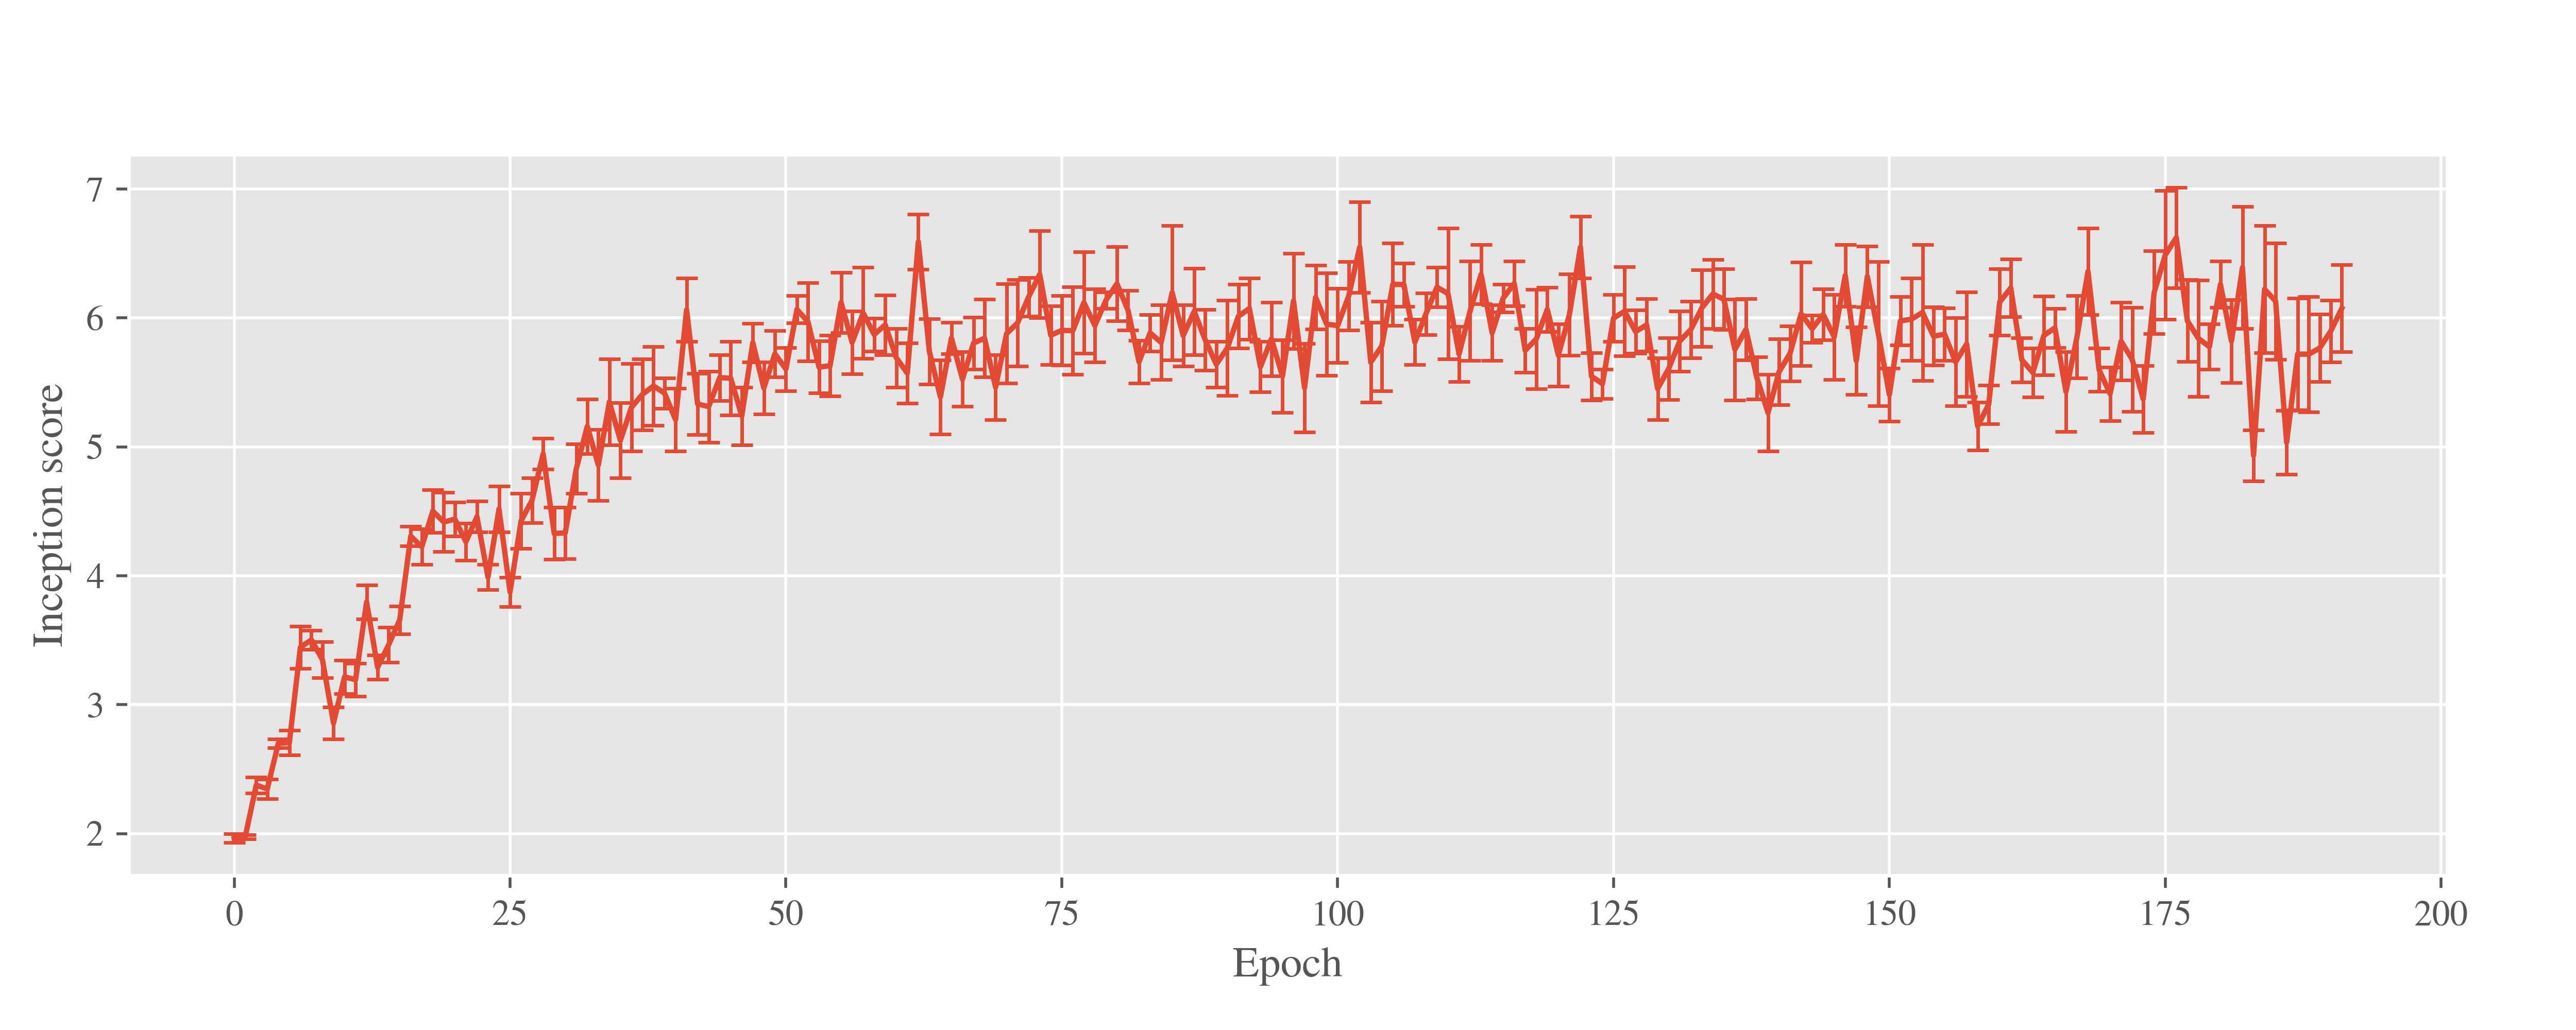
\includegraphics[width=\textwidth]{../code/results/figures/vanilla_gan_is.png}
\caption{Inception score over 190 epochs with Vanilla DCGAN.}
\label{fig:example}
\end{figure}


\begin{figure}
\centering
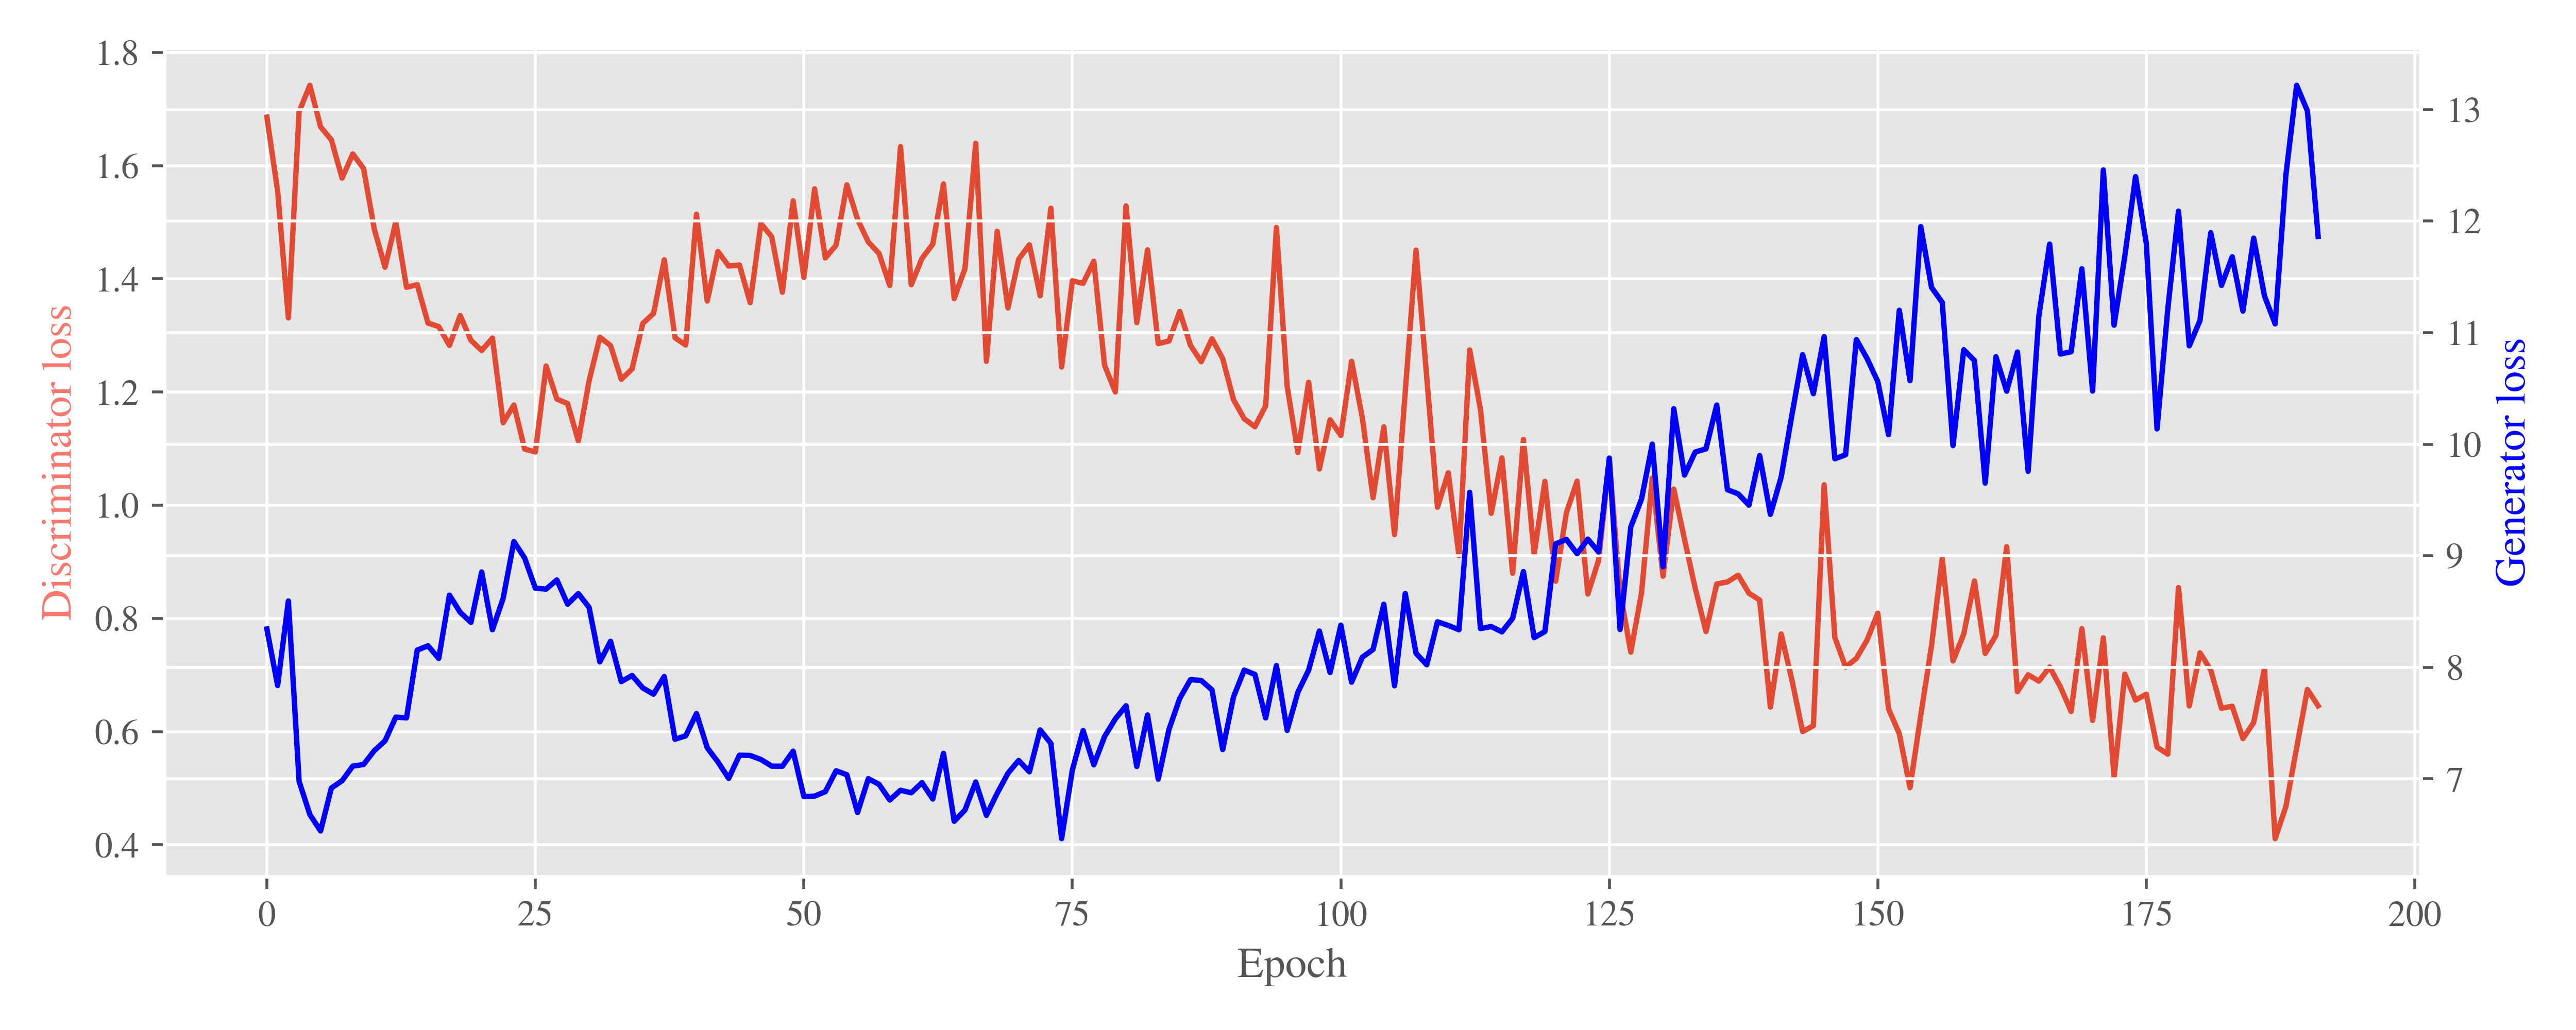
\includegraphics[width=\textwidth]{../code/results/figures/vanilla_gan_losses.png}
\caption{Losses over 190 epochs with Vanilla DCGAN.}
\label{fig:example}
\end{figure}
Unfortunately we can hardly interpret the losses of GANs, since the generator and discriminator are in a situation of competition where an improvement on the one leads to a deterioration on the other. Consequently, there exists a number of approaches to try and make these networks reach an equilibrium quicker. \todo{insert citations or examples if not already done in background theory}. However, this aspect of the art of training GANs goes below the scope of our work.

\subsection{DCGAN with Spectral Normalization}

\subsection{LSGAN}

\subsection{WGAN}